\chapter[Einleitung]{Einleitung}\label{sec:einleitung}
%\begin{tikzpicture} 
%	\begin{axis}[ 
%		xlabel=Bild, 
%		ylabel=Metrik,
%	 	axis x line*=bottom,
%	 	axis y line*=left,
%	 	ymajorgrids,
%	 	ymin=0,
%	 	ymax=1
%	] 
%	 \addplot [
%	 	color=blue,
%       ultra thick,
%      point meta=x, % Define the value that's used to determine the color
%        mark=x
%    ] coordinates { 
%	(1, 1) 
%	(2, 0.689128518) 
%	(3, 0.313492749)
%	(4, 0.197890621)
%	(5, 0.155663954)
%	(6, 0.135560304)
%	(7, 0.125045233)
%	(8, 0.119600855)
%	(9, 0.114321953)
%	(10, 0.112258035)
%	}; 
%	\end{axis} 
%\end{tikzpicture}



\section[Motivation]{Motivation}\label{sec:motivation}
Knochenmarkanalysen werden im klinischen Alltag in den verschiedensten F�llen angefordert, z.B. bei Verdacht auf Leuk�mie, da es sich hierbei um eine Erkrankung des Knochenmarks handelt. Die Krankheit kann in allen Altersgruppen auftreten, es wird zwischen den folgenden, h�ufigsten, Formen je nach Verlauf und urs�chlichem Zelltyp unterschieden:
\begin{itemize}
\item{Akute myeloische Leuk�mie (AML)}
\item{Chronische myeloische Leuk�mie (CML)}
\item{Akute lymphatische Leuk�mie (ALL)}
\item{Chronische lymphatische Leuk�mie (CLL)}
\end{itemize}
Im Kindesalter tritt fast immer ein akuter Verlauf auf, am h�ufigsten wird eine ALL diagnostiziert. Unabh�ngig vom Alter bildet jedoch die CLL mit �ber einem Drittel die zahlreichste Form. Im Jahr 2012 lag die Zahl der Neuerkrankungen an Leuk�mie bei ca. 12640 F�llen, 5\% davon unter 15 Jahren. Eine �bersicht �ber das Alter der neuerkrankten Patienten zeigt Abbildung \ref{fig:leukemia_age}. Aus dieser Statistik geht ebenfalls hervor, dass vor allem im Erwachsenenalter M�nner h�ufiger betroffen sind als Frauen.
\begin{figure}
\center
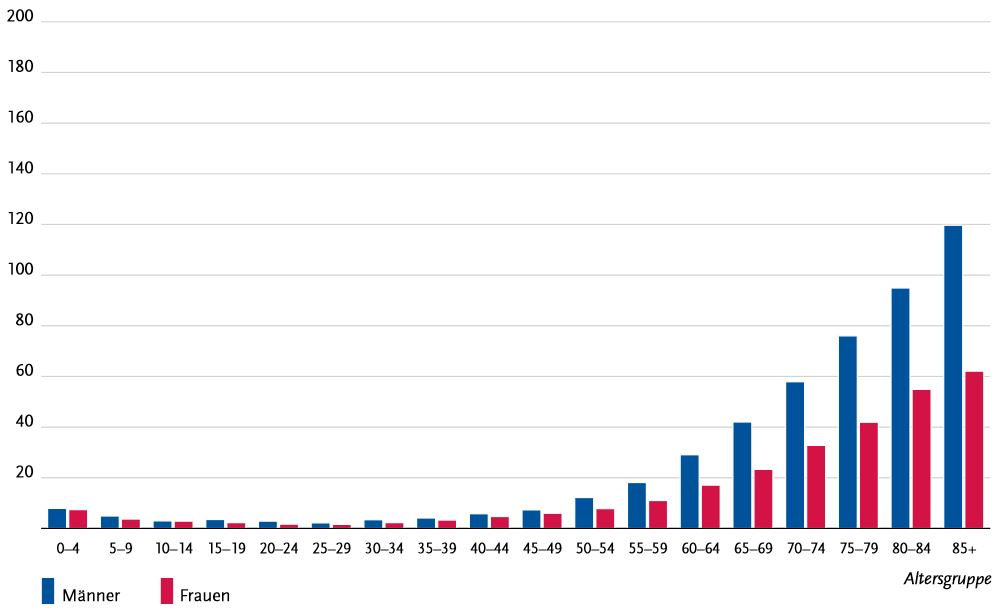
\includegraphics[width = 0.9\textwidth]{pics/Einleitung/leukaemie_statistic_age}
\caption[Neuerkrankungen Leuk�mie nach Alter und Geschlecht]{Die Graphik zeigt die Statistik der Neuerkrankungen mit Leuk�mie in Deutschland f�r die Jahre 2011 und 2012 nach Alter (horizontale Achse) und Geschlecht (Balkenfarbe). Die Zahlen sind dabei relativ je 100.000 normiert \cite{url_leukemia_statistic}.\label{fig:leukemia_age}}
\end{figure}
Bei Kindern ist die Prognose deutlich g�nstiger als bei Erwachsenen. Die 5-Jahres �berlebenschance wird f�r sie mit bis zu 90\% angegeben, der Wert f�r die Erwachsenen liegt nur bei 35-50\%. Eine dauerhafte Heilung ist m�glich, es gibt sie aber nur selten z.B. durch Stammzellentransplantation. �ber die Ursachen von Leuk�mie ist indes wenig bekannt. Als Risikofaktoren gelten ionisierende Strahlung, z.B. bei Strahlen- oder Chemotherapie, und der Umgang mit Chemikalien wie Benzol. Diese Faktoren treffen aber nur auf eine kleine Gruppe der Erkrankten zu, weshalb weitere Faktoren diskutiert werden, ohne dass diese bis jetzt nachgewiesen werden konnten. Hierzu geh�ren Ern�hrungsgewohnheiten und Lebensstil, vor allem beim chronischen Verlauf, ein Einfluss von Viren und ein ungen�gendes Training des Immunsystem bei Heranwachsenden \cite{url_leukemia_statistic}.
Eine Leuk�mie macht sich in Proben des Knochenmarks dadurch bemerkbar, dass die Leukozytenzahl zugunsten anderer Zelltypen deutlich zunimmt, was Blutarmut und Probleme bei der Gerinnung zur Folge haben kann. F�r den Nachweis muss daher eine repr�sentative Anzahl an Zellen einer Klasse zugeordnet und gez�hlt werden. Dieser Vorgang ist zeitaufwendig und nicht standardisiert, weshalb es zu Abweichungen bei der Analyse durch verschiedene H�matologen kommen kann. Bei der wiederholten Auswertung durch den gleichen Arzt treten ebenfalls Diskrepanzen auf.
Das Ziel eines Projekts am Fraunhofer-Institut f�r Integrierte Schaltungen IIS ist es deshalb, den Prozess der Differentialz�hlung zu automatisieren, wodurch Ressourcen gespart werden k�nnen und eine bessere Vergleichbarkeit erzielt wird. Hierzu wurden Algorithmen entwickelt, um Zellen in gef�rbten Ausstrichen zu detektieren, zu segmentieren und zu klassifizieren. Diese Aufgabe wird dadurch erschwert, dass die Pr�parierung zwar Standards unterliegt, sich das Erscheinungsbild aber abh�ngig von Probendicke, Farbmenge, verwendetem Mikroskop usw. unterscheidet.
 
\section[Aufgabenstellung]{Aufgabenstellung}\label{sec:aufgabenstellung}
Das Ziel der vorliegenden Arbeit ist es, verschiedene Ans�tze zur Farbnormalisierung zu entwickeln, zu implementieren und miteinander zu vergleichen. Zun�chst soll hierf�r eine Literaturrecherche �ber g�ngige Verfahren sowie deren Eignung f�r das vorliegende Problem durchgef�hrt werden. Bestehende Verfahren sollen umgesetzt und gegebenenfalls angepasst und erweitert werden. Der Fokus der Evaluierung liegt auf dem Einfluss auf die Qualit�t der vorhandenen Segmentierungs- und Klassifikationsalgorithmen f�r Knochenmarkzellen. 
